% coding:utf-8

\section{Schaltung}

\subsection{Schema}
\begin{figure}[h!]
	\centering
	\includegraphics[scale=\schscale]{fig/xlr_pegelwandler_v_1_1_sch.pdf}
	\caption{Schema}
	\label{sch:pegw}
\end{figure}

\subsection{Funktion}
Die beiden Kanäle sind identisch aufgebaut. Nachfolgend wird die Funktionsweise anhand der Teilschaltung 10x gezeigt. R101 fungiert als Pull-Up Widerstand. Um Störungen durch das lange Kabel des an CON101 angeschlossenen Tasters zu verringern ist dieser relativ niederohmig ausgeführt. C101 filtert hochfrequente Störungen und stellt einen gewissen Schutz der Basis von V101 gegen ESD dar. R105 begrenzt den Strom durch die Basis von V101. Wird nun der Taster gedrückt, wird fliesst Strom durch die Basis von V101, worauf dieser beginnt zu leiten. Dadurch fliesst Strom in die Basis von V102. Dies bewirkt, dass V102 leitet. Dadurch wird das Ausgangssignal der Schaltung nach GND gezogen. Wird der Taster wieder losgelassen, sperrt V101, worauf auch V102 sparrt. Das Ausgangssignal wird durch R104 zur Betriebsspannung des Controllers gezogen. 

Aufgrund des geringeren Schaltungsaufwandes von Variante 2 wird mit dieser weiter verfahren. 

\subsubsection{Dimensionierung}
\[ \begin{matrix} R101 = \frac{U_B}{I_{sw}}\\
U_B = 6.6 V\\
I_{sw} = 20 mA\\
\Rightarrow R101 = \frac{6.6V}{20mA} = 330 \Omega
\end{matrix} \]

\subsection{Layout}
\begin{figure}[h!]
	\centering
	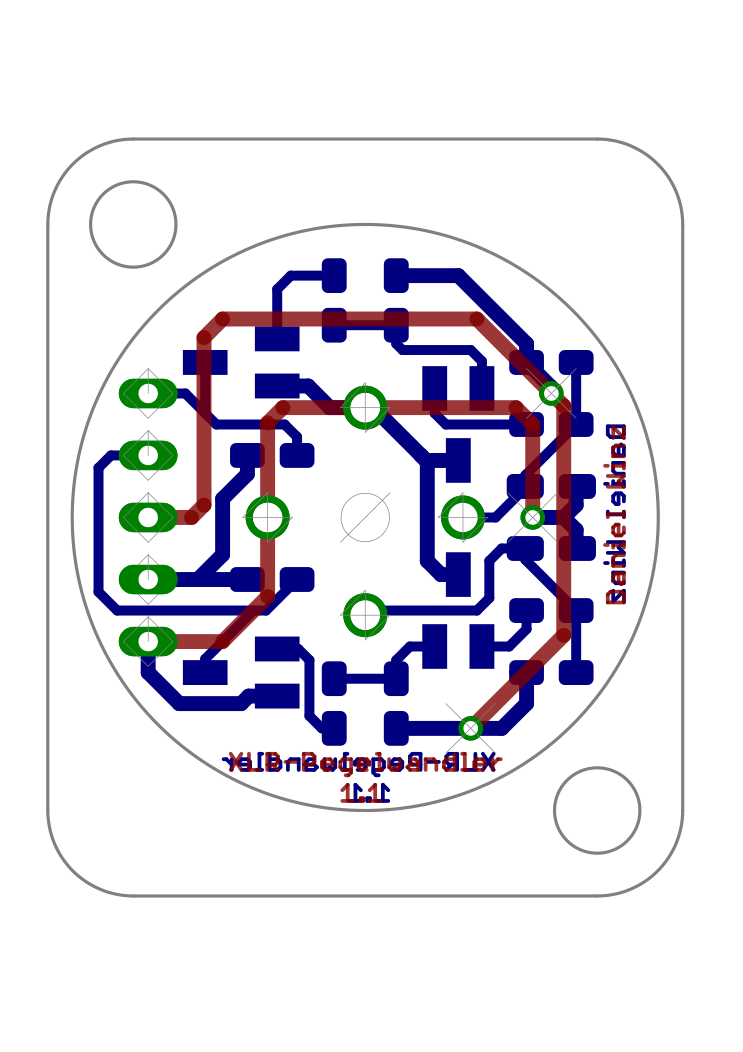
\includegraphics[scale=\schscale]{fig/xlr_pegelwandler_v_1_1_lay_transp.pdf}
	\caption{Layout}
	\label{lay:pegw}
\end{figure}
